\section{Subsample Shift}
\label{sec:02_subsampleShift}

Considering the case that the sample frequency $f_s$ is set to 44.1\si{\kilo\hertz}
and the sound speed is 343\si{m/s}, the maximum number of samples
between the rear channels is 14.
Other neighboring pairs have even less maximum sample differences.
This leads to a very low resolution of the direction angle which can be
circumvented by either setting a higher resolution or interpolation.

Quadratic interpolation is a well known technique to obtain a floating number
shift from a correlation.
For this, a parabola $y(x) = a(x-p)^2+b$ is fitted into the three values of $R$ around the peak
of the \ac{CC} and the peak of the parabola is taken as the more accurate
delay.
Thus, the subsample delay $D_{sub}$ depends on the maximum value of the correlation $y_m$
and its previous one $y_{m-1}$ and the next value $y_{m+1}$.
Substituting known values and derivations into the parabola function,
the subsample delay is defined as
\bal
	D_{sub} = \frac{y_{m-1} - y_{m+1}}{2 \cdot (y_{m-1} - 2y_{m} + y_{m+1})}
	\label{eq:02_subsample}
\eal
like in \cite{C_H_subsampleDelay}.
% -------------------------------------------------------------
\Cref{fig:02_subsampleShift} illustrates the \ac{CC} of two generated sine signals with 3\si{\kilo\hertz}.
The second signal is shifted by $\frac{\pi}{3}$ which are 2.449 samples for a sample rate
of 44.1kHz.
As the plot shows, the peak of the parabola can be determined at an index of 2.446 by
quadratic interpolation.
\begin{figure}[ht]
	\centering
		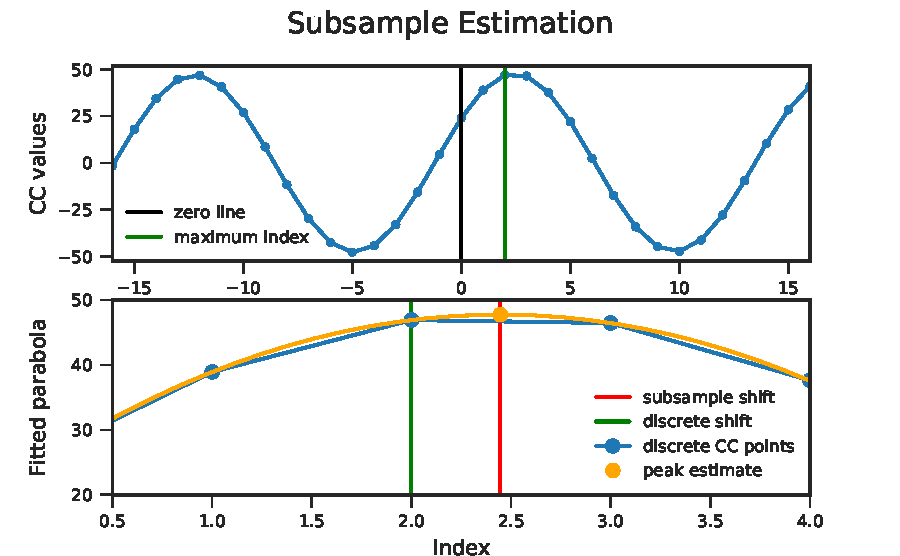
\includegraphics[]{figures/subsample_shift}
	\caption{Explanation example of the subsample shift estimation using parabolic interpolation.}
    \label{fig:02_subsampleShift}
\end{figure}
% -------------------------------------------------------------
In research there are efforts in finding a better approximation function than the quadratic as stated
in \cite{S_L_subsampleInterpolation} but these are not discussed in greater detail here
due to sufficiency.
% -------------------------------------------------------------
% index = 2 -> -14.6deg
% index = 3 -> -22.2deg
% index = 2.445 -> -17.9deg